\documentclass[10pt,letterpaper]{article}

\usepackage[letterpaper,left=0.65in,right=0.65in,top=0.72in,bottom=0.72in,headheight=19pt]{geometry}
\usepackage{fontspec}
\usepackage{amsmath,amssymb}
\usepackage{graphicx}
\usepackage{booktabs}
\usepackage{longtable}
\usepackage{array}
\usepackage{xcolor}
\usepackage{titlesec}
\usepackage{fancyhdr}
\usepackage{lastpage}
\usepackage[hidelinks]{hyperref}
\urlstyle{same}

\setmainfont{Arial}[
  Scale=0.92,
  BoldFont={Arial Bold},
  ItalicFont={Arial Italic},
  BoldItalicFont={Arial Bold Italic}
]
\setsansfont{Arial}[Scale=0.92]
\setmonofont{Arial}[Scale=0.92]

\linespread{1.08}
\setlength{\parindent}{0pt}
\setlength{\parskip}{4pt}
\definecolor{RuleGray}{HTML}{BDBDBD}
\color{black}

\titleformat{\section}
  {\fontsize{11.5}{14}\selectfont\bfseries\color{black}}
  {}{0pt}{}
  [\vspace{-3pt}\textcolor{RuleGray}{\rule{\textwidth}{0.5pt}}]
\titlespacing*{\section}{0pt}{12pt}{6pt}

\pagestyle{fancy}
\fancyhf{}
\renewcommand{\headrulewidth}{0.4pt}
\renewcommand{\headrule}{\hbox to\headwidth{\color{RuleGray}\leaders\hrule height \headrulewidth\hfill}}
\fancyhead[L]{\footnotesize\color{black}Koppikar (2026) \textbar\ Supplementary Information: Pan-prokaryotic +1 overprinted C5-MTase family}
\fancyhead[R]{\footnotesize\color{black}Supplementary Information}
\fancyfoot[C]{\footnotesize\color{black}S\thepage\ / S\pageref{LastPage}}

\newcommand{\gene}[1]{\textit{#1}}
\newcommand{\spname}[1]{\textit{#1}}

\begin{document}

\noindent{\fontsize{13.5}{17}\selectfont\bfseries\color{black}\raggedright
Supplementary Information\\[3pt]
A Pan-Prokaryotic and Viral +1 Overprinted Gene Family Inside Full-Length C5-Cytosine DNA Methyltransferases Explains the Origin of Split-Subunit Methyltransferases\par}
\vspace{4pt}
\noindent{\small Pratik Koppikar\textsuperscript{1,*} \;\textbar\; \textsuperscript{1}University of Cambridge, Cambridge, United Kingdom \;\textbar\; \href{mailto:psk34@cam.ac.uk}{psk34@cam.ac.uk}\\
Repository and raw datasets: \url{https://github.com/koppikarp/c5mtase-plus1-overprint}\par}
\vspace{3pt}
\noindent{\color{RuleGray}\rule{\textwidth}{0.7pt}}

\section*{Contents}
\begin{itemize}
  \item \textbf{Supplementary Figure S1:} Full uncollapsed maximum-likelihood phylogenies of Frame-0 C5-MTases (Tree 1, $n=97$ taxa) and the CSLSDILE/KYFLS domain (Tree 2, $n=67$ taxa).
  \item \textbf{Supplementary Table S1:} Complete census of all 45 verified GTDB R232 loci across 13 prokaryotic phyla.
  \item \textbf{Supplementary Table S2:} Complete census of all 39 INPHARED bacteriophage C5-MTase +1 loci and dereplicated prevalence.
  \item \textbf{Supplementary Table S3:} UniRef100/UniProtKB database erasure audit ($n=33$) and DNA-level reading-frame audit of UniProt TPCQ entries ($n=6$).
  \item \textbf{Supplementary Table S4:} Complete summary of evolutionary selection, stop-purging, phylogenetic support, Mantel congruence, and sensitivity checks.
  \item \textbf{Supplementary Table S5:} Per-model AlphaFold 3 benchmark across all 30 diffusion models (6 complexes $\times$ 5 models).
\end{itemize}

\newpage
\section*{Supplementary Figure S1}
\begin{figure}[!htbp]
  \centering
  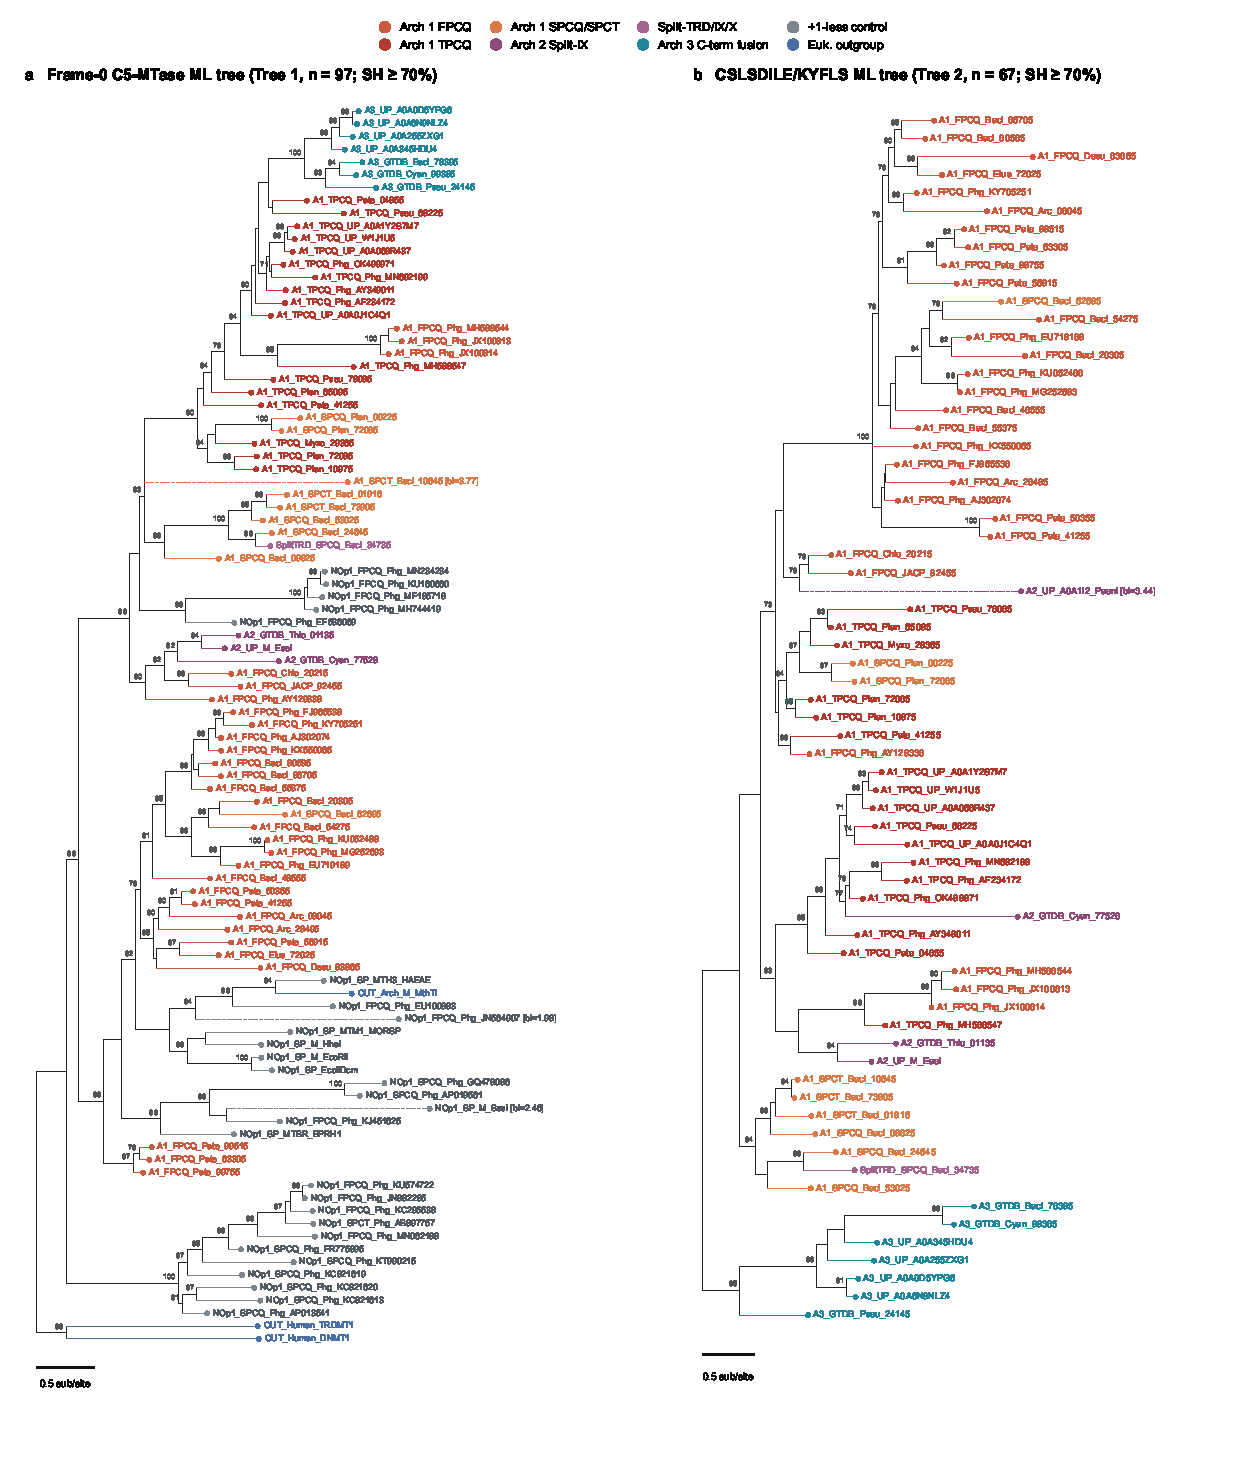
\includegraphics[width=\textwidth,height=0.81\textheight,keepaspectratio]{figures/rendered/supp_fig1_full_trees.pdf}
  \par\vspace{6pt}
  \noindent\begin{minipage}{\textwidth}\footnotesize\raggedright
  \textbf{Supplementary Figure S1. Full uncollapsed maximum-likelihood phylogenies supporting Figure 3.} \textbf{a}, Complete DNMT1/TRDMT1-rooted LG+$\Gamma$ ML phylogeny of the Frame-0 C5-MTase catalytic core (Tree 1; 97 unique non-redundant taxa, 185 MAFFT L-INS-i columns). The extreme long-branch taxon \texttt{A1\_SPCT\_Baci\_10645} (branch length 3.77) is truncated visually with a dashed branch and annotated with its true length; removing this taxon in sensitivity re-inference (96 taxa, 100 thorough ML bootstraps) yields Arch 3 monophyly ML 99\% / SH 99.6\% and TPCQ+Arch 3 superclade ML 95\% / SH 100.0\%. \textbf{b}, Complete harmonized LG+$\Gamma$ ML phylogeny of the CSLSDILE/KYFLS domain (Tree 2; 67 taxa, 77 trimmed columns), rooted on the monophyletic Arch 3 C-terminal fusion clade for display. Numbers at internal nodes show SH-like local support values ($\ge 70\%$).
  \end{minipage}
\end{figure}

\newpage
\section*{Supplementary Table S1: Complete Census of All 45 Verified GTDB R232 Loci}
{\scriptsize\setlength{\tabcolsep}{3.2pt}\renewcommand{\arraystretch}{1.10}
\begin{longtable}{@{}llllllllll@{}}
\toprule
\textbf{Genome} & \textbf{Domain} & \textbf{Phylum} & \textbf{Order} & \textbf{Motif IV} & \textbf{Architecture} & \textbf{F0 aa} & \textbf{+1 aa} & \textbf{GC\%} & \textbf{Motif IX} \\
\midrule
\endfirsthead
\toprule
\textbf{Genome} & \textbf{Domain} & \textbf{Phylum} & \textbf{Order} & \textbf{Motif IV} & \textbf{Architecture} & \textbf{F0 aa} & \textbf{+1 aa} & \textbf{GC\%} & \textbf{Motif IX} \\
\midrule
\endhead
\bottomrule
\endfoot
GCA\_964428495.1 & Archaea & Aenigmatarchaeota & GW2011-AR5 & FPCQ & Arch 1 (intact) & 372 & 192 & 35.5 & Frame 0 \\
GCA\_000019165.1 & Bacteria & Bacillota & Heliobacteriales & SPCT & Arch 1 (intact) & Full & 135 & 58.0 & Frame 0 \\
GCA\_000510645.1 & Bacteria & Bacillota & Thermicanales & SPCT & Arch 1 (intact) & Full & 135 & 49.1 & Frame 0 \\
GCA\_000620305.1 & Bacteria & Bacillota & Desulfitibacterales & FPCQ & Arch 1 (intact) & 440 & 165 & 39.8 & Frame 0 (div.) \\
GCA\_002224645.1 & Bacteria & Bacillota & Dehalobacteriales & SPCQ & Arch 1 (intact) & 752 & 144 & 44.2 & Frame 0 \\
GCA\_002355375.1 & Bacteria & Bacillota & Aneurinibacillales & FPCQ & Arch 1 (intact) & 389 & 164 & 46.8 & Frame 0 \\
GCA\_005473905.2 & Bacteria & Bacillota & Acetivibrionales & SPCT & Arch 1 (intact) & Full & 136 & 34.5 & Frame 0 \\
GCA\_005848555.1 & Bacteria & Bacillota & Lachnospirales & FPCQ & Arch 1 (intact) & 447 & 204 & 45.0 & Frame 0 \\
GCA\_031554275.1 & Bacteria & Bacillota & JARBTR01 & FPCQ & Arch 1 (intact) & 350 & 166 & 39.5 & Frame 0 \\
GCA\_033880585.1 & Bacteria & Bacillota & Bacillales\_A & FPCQ & Arch 1 (intact) & 413 & 163 & 39.2 & Frame 0 \\
GCA\_048453025.1 & Bacteria & Bacillota & Thermincolales & SPCQ & Arch 1 (intact) & 636 & 134 & 43.1 & Frame 0 \\
GCA\_900086705.1 & Bacteria & Bacillota & FLKF01 & FPCQ & Arch 1 (intact) & 365 & 161 & 38.6 & Frame 0 \\
GCA\_902809825.1 & Bacteria & Bacillota & Sulfobacillales & SPCQ & Arch 1 (intact) & 548 & 279 & 70.9 & Frame 0 \\
GCA\_963662695.2 & Bacteria & Bacillota & SK-Y3 & SPCQ & Arch 1 (intact) & 462 & 168 & 34.2 & Frame 0 (div.) \\
GCA\_965220215.1 & Bacteria & Chloroflexota & SHYD01 & FPCQ & Arch 1 (intact) & 326 & 188 & 60.8 & Frame 0 \\
GCA\_030583865.1 & Bacteria & Desulfobacterota & GWC2-55-46 & FPCQ & Arch 1 (intact) & 385 & 194 & 58.8 & Frame 0 \\
GCA\_022072025.1 & Bacteria & Elusimicrobiota & F11 & FPCQ & Arch 1 (intact) & 440 & 219 & 49.0 & Frame 0 \\
GCA\_016192455.1 & Bacteria & JACPUC01 & JACPUC01 & FPCQ & Arch 1 (intact) & 344 & 155 & 67.0 & Frame 0 (div.) \\
GCA\_023229365.1 & Bacteria & Myxococcota\_A & JAAYKL01 & TPCQ & Arch 1 (intact) & 440 & 185 & 64.9 & Frame 0 \\
GCA\_017608045.1 & Archaea & Nanobdellota & JAFCGN01 & FPCQ & Arch 1 (intact) & 405 & 236 & 29.8 & Frame 0 \\
GCA\_016699515.1 & Bacteria & Patescibacteriota & UM-FILTER-43-11 & FPCQ & Arch 1 (intact) & 472 & 143 & 46.4 & Frame 0 \\
GCA\_016699755.1 & Bacteria & Patescibacteriota & CAIRYL01 & FPCQ & Arch 1 (intact) & 340 & 182 & 41.4 & Frame 0 \\
GCA\_963663305.1 & Bacteria & Patescibacteriota & G963663305 & FPCQ & Arch 1 (intact) & 319 & 183 & 31.8 & Frame 0 \\
GCA\_964356915.1 & Bacteria & Patescibacteriota & Ryanbacterales & FPCQ & Arch 1 (intact) & 404 & 259 & 45.2 & Frame 0 \\
GCA\_964404855.1 & Bacteria & Patescibacteriota & CAYQLK01 & TPCQ & Arch 1 (intact) & 499 & 150 & 44.0 & Frame 0 \\
GCA\_964641255.1 & Bacteria & Patescibacteriota & JAMCZE01 & FPCQ & Arch 1 (intact) & 423 & 241 & 48.0 & Frame 0 \\
GCA\_964641255.1 & Bacteria & Patescibacteriota & JAMCZE01 & TPCQ & Arch 1 (intact) & 403 & 206 & 48.0 & Frame 0 \\
GCA\_964650355.1 & Bacteria & Patescibacteriota & CAYXHB01 & FPCQ & Arch 1 (intact) & 365 & 206 & 44.9 & Frame 0 \\
GCA\_008065095.1 & Bacteria & Planctomycetota & Gemmatales & TPCQ & Arch 1 (intact) & 489 & 201 & 68.0 & Frame 0 \\
GCA\_022072085.1 & Bacteria & Planctomycetota & JAJVII01 & TPCQ & Arch 1 (intact) & 583 & 165 & 68.2 & Frame 0 \\
GCA\_022072085.1 & Bacteria & Planctomycetota & JAJVII01 & SPCQ & Arch 1 (intact) & 694 & 178 & 68.2 & Frame 0 (div.) \\
GCA\_964500225.1 & Bacteria & Planctomycetota & FEN-1346 & SPCQ & Arch 1 (intact) & 630 & 167 & 65.4 & Frame 0 \\
GCA\_964610975.1 & Bacteria & Planctomycetota & WQYP01 & TPCQ & Arch 1 (intact) & 409 & 167 & 53.9 & Frame 0 \\
GCA\_002168225.1 & Bacteria & Pseudomonadota & TMED2 & TPCQ & Arch 1 (intact) & 459 & 136 & 59.2 & Frame 0 (div.) \\
GCA\_965178085.1 & Bacteria & Pseudomonadota & CBCXTS01 & TPCQ & Arch 1 (intact) & 409 & 159 & 39.3 & Frame 0 \\
GCA\_041653515.1 & Archaea & Nanobdellota & WJKC01 & FPCQ & Arch 1 (interrupted) & -- & 203 & 36.6 & Frame 0 \\
GCA\_963663305.1 & Bacteria & Patescibacteriota & G963663305 & FPCQ & Arch 1 (interrupted) & -- & 148 & 31.8 & Frame 0 \\
GCA\_000775285.1 & Bacteria & Cyanobacteriota & Neosynechococcales & WPCQ & Arch 2 (split IX) & Full & 257 & 52.5 & Frame +1 \\
GCA\_017901135.1 & Bacteria & Pseudomonadota & Thiotrichales & FPCQ & Arch 2 (split IX) & 314 & 186 & 53.5 & Frame +1 \\
GCA\_963678395.1 & Bacteria & Bacillota & Acidaminococcales & TPCQ/fusion & Arch 3 (C-term fusion) & 457 & In-frame & 38.6 & Frame 0 \\
GCA\_023151185.1 & Bacteria & Bacteroidota & JABWAT01 & TPCQ/fusion & Arch 3 (C-term fusion) & 452 & In-frame & 48.2 & Frame 0 \\
GCA\_001899385.1 & Bacteria & Cyanobacteriota & Caenarcaniphilales & TPCQ/fusion & Arch 3 (C-term fusion) & 472 & In-frame & 26.4 & Frame 0 \\
GCA\_012224145.1 & Bacteria & Pseudomonadota & Francisellales & TPCQ/fusion & Arch 3 (C-term fusion) & 409 & In-frame & 32.5 & Frame 0 \\
GCA\_035934735.1 & Bacteria & Bacillota & Tissierellales & SPCQ & Split TRD/IX/X & 223 & 120 & 30.5 & Frame +1 (TRD--X) \\
GCA\_035934735.1 & Bacteria & Bacillota & Tissierellales & SPCQ & Split TRD/IX/X & 224 & 120 & 30.5 & Frame +1 (TRD--X) \\
\end{longtable}
}

\newpage
\section*{Supplementary Table S2: Complete Census of All 39 INPHARED Bacteriophage +1 Loci}
\noindent{\footnotesize Dereplicated phage prevalence across all 230 C5-MTases: $<95\%$ identity: 18/121 clusters (14.9\%); $<90\%$ identity: 15/109 clusters (13.8\%, TPCQ 5/6 [83.3\%], FPCQ 10/47 [21.3\%]); $<80\%$ identity: 11/92 clusters (12.0\%, TPCQ 5/6 [83.3\%]).\par}
\vspace{4pt}
{\scriptsize\setlength{\tabcolsep}{4.2pt}\renewcommand{\arraystretch}{1.10}
\begin{longtable}{@{}lllllllll@{}}
\toprule
\textbf{GenBank Acc.} & \textbf{Motif IV} & \textbf{Architecture} & \textbf{Frame-0 aa} & \textbf{+1 ORF aa} & \textbf{Frame-0 IX} & \textbf{Frame-0 X} & \textbf{GC\%} & \textbf{Seed ID\%} \\
\midrule
\endfirsthead
\toprule
\textbf{GenBank Acc.} & \textbf{Motif IV} & \textbf{Architecture} & \textbf{Frame-0 aa} & \textbf{+1 ORF aa} & \textbf{Frame-0 IX} & \textbf{Frame-0 X} & \textbf{GC\%} & \textbf{Seed ID\%} \\
\midrule
\endhead
\bottomrule
\endfoot
AJ302074 & FPCQ & Arch 1 (intact) & 385 & 161 & Yes & Yes & 38.4 & 61.7 \\
DQ466086 & FPCQ & Arch 1 (intact) & 333 & 154 & Yes & No & 28.7 & 42.9 \\
FJ965538 & FPCQ & Arch 1 (intact) & 319 & 143 & Yes & Yes & 38.0 & 60.8 \\
HG531805 & FPCQ & Arch 1 (intact) & 357 & 154 & Yes & Yes & 28.4 & 42.9 \\
JX100809 & FPCQ & Arch 1 (intact) & 352 & 154 & Div/Split & Yes & 66.1 & 34.5 \\
JX100813 & FPCQ & Arch 1 (intact) & 352 & 154 & Div/Split & Yes & 66.2 & 34.5 \\
JX100814 & FPCQ & Arch 1 (intact) & 357 & 145 & Div/Split & Yes & 66.1 & 43.7 \\
JX145341 & FPCQ & Arch 1 (intact) & 357 & 154 & Yes & Yes & 29.6 & 42.9 \\
KU052488 & FPCQ & Arch 1 (intact) & 374 & 161 & Yes & Yes & 37.5 & 39.7 \\
KX228399 & FPCQ & Arch 1 (intact) & 357 & 154 & Yes & Yes & 29.0 & 42.9 \\
KX228400 & FPCQ & Arch 1 (intact) & 357 & 154 & Yes & Yes & 28.7 & 42.9 \\
KX550065 & FPCQ & Arch 1 (intact) & 377 & 160 & Yes & Yes & 38.3 & 54.4 \\
KX879643 & FPCQ & Arch 1 (intact) & 287 & 141 & Yes & Yes & 38.5 & 100.0 \\
KY065455 & FPCQ & Arch 1 (intact) & 377 & 160 & Yes & Yes & 38.4 & 54.4 \\
KY065487 & FPCQ & Arch 1 (intact) & 412 & 160 & Yes & Yes & 38.5 & 53.7 \\
KY065490 & FPCQ & Arch 1 (intact) & 363 & 160 & Yes & Yes & 38.1 & 52.3 \\
KY065493 & FPCQ & Arch 1 (intact) & 383 & 165 & Yes & Yes & 38.7 & 51.7 \\
KY705251 & FPCQ & Arch 1 (intact) & 287 & 141 & Yes & Yes & 39.2 & 100.0 \\
KY705252 & FPCQ & Arch 1 (intact) & 287 & 141 & Yes & Yes & 38.4 & 99.3 \\
KY705253 & FPCQ & Arch 1 (intact) & 287 & 141 & Yes & Yes & 38.6 & 100.0 \\
KY705255 & FPCQ & Arch 1 (intact) & 287 & 141 & Yes & Yes & 38.1 & 99.3 \\
LK985322 & FPCQ & Arch 1 (intact) & 357 & 154 & Yes & Yes & 28.2 & 42.9 \\
LN681539 & FPCQ & Arch 1 (intact) & 357 & 154 & Yes & Yes & 29.4 & 42.9 \\
LN681542 & FPCQ & Arch 1 (intact) & 357 & 154 & Yes & Yes & 28.9 & 42.9 \\
MG252693 & FPCQ & Arch 1 (intact) & 394 & 161 & Yes & Yes & 37.2 & 41.5 \\
MH588544 & FPCQ & Arch 1 (intact) & 357 & 152 & Div/Split & Yes & 65.7 & 39.1 \\
MH937506 & FPCQ & Arch 1 (intact) & 287 & 141 & Yes & Yes & 38.0 & 100.0 \\
MK202161 & FPCQ & Arch 1 (intact) & 287 & 141 & Yes & Yes & 38.1 & 100.0 \\
AY129338 & FPCQ & Arch 1 (interrupted) & 247 & 159 & Div/Split & No & 61.4 & 37.3 \\
AY855346 & FPCQ & Arch 1 (interrupted) & 260 & 154 & Div/Split & No & 28.8 & 42.9 \\
EU719189 & FPCQ & Arch 1 (interrupted) & 276 & 154 & Div/Split & No & 29.3 & 42.9 \\
KY065492 & FPCQ & Arch 1 (interrupted) & 260 & 160 & Div/Split & No & 38.4 & 54.4 \\
AF234172 & TPCQ & Arch 1 (intact) & 754 & 163 & Yes & No & 47.3 & 44.9 \\
AY349011 & TPCQ & Arch 1 (intact) & 370 & 156 & Div/Split & Yes & 65.3 & 62.1 \\
KU760857 & TPCQ & Arch 1 (intact) & 807 & 166 & Yes & No & 48.6 & 43.1 \\
MH588546 & TPCQ & Arch 1 (intact) & 328 & 149 & Div/Split & Yes & 63.7 & 44.6 \\
MH588547 & TPCQ & Arch 1 (intact) & 328 & 149 & Div/Split & Yes & 64.2 & 45.5 \\
MN692199 & TPCQ & Arch 1 (intact) & 507 & 172 & Div/Split & Yes & 54.5 & 54.9 \\
OK499971 & TPCQ & Arch 1 (intact) & 637 & 145 & Yes & No & 52.7 & 58.1 \\
\end{longtable}
}

\newpage
\section*{Supplementary Table S3: Database Erasure Audit and DNA-Level Verification}
\noindent{\footnotesize\textbf{Table S3a.} All 33 audited non-UniParc UniProtKB matches among top MMseqs2 UniRef100 hits (query: \spname{Aneurinibacillales} +1 polypeptide, GCA\_002355375.1): 29/33 (87.9\%) marked deleted/obsolete; 4/33 active, all with 0 Pfam and 0 InterPro hits.\par}
\vspace{3pt}
{\scriptsize\setlength{\tabcolsep}{3.5pt}\renewcommand{\arraystretch}{1.08}
\begin{longtable}{@{}rlllrrll@{}}
\toprule
\textbf{Rank} & \textbf{Accession} & \textbf{UniProtKB Status} & \textbf{ID\%} & \textbf{Q.Cov.} & \textbf{E-value} & \textbf{Organism (if active)} & \textbf{Pfam / InterPro} \\
\midrule
\endfirsthead
\toprule
\textbf{Rank} & \textbf{Accession} & \textbf{UniProtKB Status} & \textbf{ID\%} & \textbf{Q.Cov.} & \textbf{E-value} & \textbf{Organism (if active)} & \textbf{Pfam / InterPro} \\
\midrule
\endhead
\bottomrule
\endfoot
1 & Q0R5A0 & deleted & 55.7\% & 90.2\% & 1.0e-40 & -- & 0 / 0 \\
2 & A0A0E0UZB9 & deleted & 47.9\% & 95.4\% & 2.7e-37 & -- & 0 / 0 \\
3 & A0A428C2B5 & deleted & 48.2\% & 90.8\% & 9.4e-37 & -- & 0 / 0 \\
4 & A0A3R9KVA1 & deleted & 50.0\% & 75.8\% & 7.7e-35 & -- & 0 / 0 \\
5 & A0A060QS82 & deleted & 41.7\% & 89.5\% & 2.5e-33 & -- & 0 / 0 \\
6 & A0A645HYN9 & deleted & 42.8\% & 87.6\% & 3.1e-32 & -- & 0 / 0 \\
7 & A0A081SA93 & deleted & 40.2\% & 89.5\% & 3.1e-32 & -- & 0 / 0 \\
8 & A0A0F9G3Z2 & deleted & 38.8\% & 86.3\% & 7.2e-31 & -- & 0 / 0 \\
9 & A0A4D6AF67 & deleted & 33.5\% & 81.0\% & 9.0e-30 & -- & 0 / 0 \\
10 & A0A0G1MCW7 & deleted & 39.8\% & 85.0\% & 9.0e-30 & -- & 0 / 0 \\
11 & D7GWH7 & deleted & 37.1\% & 83.7\% & 1.7e-29 & -- & 0 / 0 \\
12 & A0A0F9J4V1 & deleted & 39.3\% & 100.0\% & 8.2e-29 & -- & 0 / 0 \\
13 & A0A173VQH5 & deleted & 38.8\% & 98.0\% & 1.1e-28 & -- & 0 / 0 \\
14 & A0A286QMS3 & active & 49.5\% & 77.8\% & 1.4e-27 & Streptococcus phage P0093 & 0 / 0 \\
15 & G6FBV4 & deleted & 49.5\% & 79.7\% & 1.9e-27 & -- & 0 / 0 \\
16 & A0A069AZW9 & deleted & 37.6\% & 82.4\% & 9.2e-27 & -- & 0 / 0 \\
17 & A0A174U5Z5 & deleted & 44.4\% & 70.6\% & 3.2e-26 & -- & 0 / 0 \\
18 & A0A3P5XT20 & active & 50.0\% & 60.1\% & 8.3e-26 & Streptococcus canis & 0 / 0 \\
19 & A0A2M8Z2X8 & deleted & 31.1\% & 86.3\% & 1.6e-25 & -- & 0 / 0 \\
20 & A0A0C1M8B8 & deleted & 38.5\% & 85.0\% & 5.0e-24 & -- & 0 / 0 \\
21 & A0A0F9ILU5 & deleted & 35.6\% & 83.0\% & 4.5e-23 & -- & 0 / 0 \\
22 & A0A4D6B452 & deleted & 33.6\% & 67.3\% & 8.5e-23 & -- & 0 / 0 \\
23 & O52510 & active & 31.8\% & 59.5\% & 5.1e-21 & Klebsiella aerogenes & 0 / 0 \\
26 & A0A943HXC9 & deleted & 30.3\% & 51.6\% & 7.6e-13 & -- & 0 / 0 \\
27 & A0A382WDW1 & deleted & 49.2\% & 45.1\% & 2.7e-12 & -- & 0 / 0 \\
28 & R7BID8 & deleted & 36.8\% & 36.6\% & 2.7e-12 & -- & 0 / 0 \\
29 & A0A374UQL1 & deleted & 27.5\% & 41.2\% & 3.2e-11 & -- & 0 / 0 \\
30 & A0A2J4JSK0 & deleted & 36.0\% & 32.7\% & 6.1e-11 & -- & 0 / 0 \\
31 & K1UL71 & deleted & 52.0\% & 31.4\% & 1.1e-10 & -- & 0 / 0 \\
33 & A7AY33 & deleted & 55.7\% & 34.0\% & 2.1e-10 & -- & 0 / 0 \\
53 & M3AAZ1 & active & 29.7\% & 53.6\% & 2.7e-07 & Paramagnetospirillum caucaseum & 0 / 0 \\
56 & A0A7U9MVK5 & deleted & 22.5\% & 50.3\% & 9.5e-07 & -- & 0 / 0 \\
58 & A0A8D9NQQ0 & deleted & 28.1\% & 49.0\% & 2.4e-06 & -- & 0 / 0 \\
\end{longtable}
}

\vspace{8pt}
\noindent{\footnotesize\textbf{Table S3b.} DNA-level reading-frame audit of five UniProt TPCQ entries initially appearing +1-less in protein records (5/5 carry intact unannotated +1 CSLSDILE/KYFLS ORFs with 0 internal stops) plus the Arch 2 $\beta$ reference \texttt{A0A1I2CIH5}.\par}
\vspace{3pt}
{\scriptsize\setlength{\tabcolsep}{3.2pt}\renewcommand{\arraystretch}{1.10}
\begin{longtable}{@{}llllrlll@{}}
\toprule
\textbf{UniProt} & \textbf{Entry} & \textbf{Organism} & \textbf{ENA/GenBank} & \textbf{F0 aa} & \textbf{Motif IV} & \textbf{Intact +1?} & \textbf{+1 Stops} \\
\midrule
\endhead
\bottomrule
\endfoot
W1J1U5 & W1J1U5\_9GAMM & Xenorhabdus szentirmaii DSM 16338 & CDL83851.1 & 415 & TPCQ & Yes & 0 \\
A0A068R437 & A0A068R437\_9GAMM & Xenorhabdus poinarii G6 & CDG21671.1 & 347 & TPCQ & Yes & 0 \\
A0A1Y2S7M7 & A0A1Y2S7M7\_9GAMM & Xenorhabdus vietnamensis & OTA14635.1 & 413 & TPCQ & Yes & 0 \\
A0A0J1C4Q1 & A0A0J1C4Q1\_9NEIS & Neisseria arctica & KLT73288.1 & 401 & TPCQ & Yes & 0 \\
Q71TL0 & DAM\_BPP1 & Escherichia virus P1 (AF234172) & AF234172 & 754 & TPCQ & Yes & 0 \\
A0A1I2CIH5 & A0A1I2CIH5\_9BACL & Paenibacillus algorifonticola (Arch 2 +1 beta subunit itself) & SFE68179.1 & 220 & N/A\_beta\_subunit & No (beta) & 8 \\
\end{longtable}
}

\newpage
\section*{Supplementary Table S4: Evolutionary Selection, Phylogenetic Support, and Sensitivity Audit}
{\scriptsize\setlength{\tabcolsep}{3.5pt}\renewcommand{\arraystretch}{1.15}
\begin{longtable}{@{}p{0.31\textwidth}p{0.25\textwidth}p{0.24\textwidth}p{0.15\textwidth}@{}}
\toprule
\textbf{Analysis / Cohort} & \textbf{Statistical Test / Model} & \textbf{Observed Effect} & \textbf{$P$-value / Check} \\
\midrule
\endfirsthead
\toprule
\textbf{Analysis / Cohort} & \textbf{Statistical Test / Model} & \textbf{Observed Effect} & \textbf{$P$-value / Check} \\
\midrule
\endhead
\bottomrule
\endfoot
4D non-stop-risk excess (Arch 1 FPCQ, $n=13$ loci / 51 pairs) & Inside vs.\ outside (paired 1-sided Wilcoxon) & Med. $+0.258$ vs.\ $+0.015$ (13/13) & $1.22 \times 10^{-4}$ \\
4D non-stop-risk excess (Arch 1 TPCQ/SPCQ, $n=7$ loci / 12 pairs) & Inside vs.\ outside (paired 1-sided Wilcoxon) & Med. $+0.225$ vs.\ $+0.035$ (6/7) & 0.0156 \\
4D inside excess: FPCQ vs.\ +1-less controls ($n=13$ vs.\ 26) & Between-group 1-sided Mann--Whitney $U$ & Med. $+0.258$ vs.\ $+0.030$ & $2.58 \times 10^{-7}$ \\
4D inside$-$outside $\Delta$: FPCQ vs.\ controls ($n=13$ vs.\ 26) & Between-group 1-sided Mann--Whitney $U$ & Delta enrichment & $6.45 \times 10^{-7}$ \\
4D inside excess: TPCQ/SPCQ vs.\ controls ($n=7$ vs.\ 26) & Between-group 1-sided Mann--Whitney $U$ & Med. $+0.225$ vs.\ $+0.030$ & $8.19 \times 10^{-4}$ \\
4D disjoint non-overlapping pairs (200 random matchings) & Zero genome reuse (paired 1-sided Wilcoxon) & Med. frac in$>$out 83.3\% & 0.0312 \\
4D greedy disjoint FPCQ vs.\ disjoint controls (6 vs.\ 10 pairs) & Zero genome reuse (1-sided MWU) & Med. $+0.195$ inside & $2.50 \times 10^{-4}$ \\
5-frame stop purge: Frame +1 vs.\ flanking null ($n=30$ genomes) & Exact 1-sided paired Wilcoxon (1,000 null reps) & Obs. med. 0.0 vs.\ null 4.7 (30/30) & $9.31 \times 10^{-10}$ \\
5-frame stop purge: low all-codon $\text{GC3} \le 0.45$ ($n=14$) & Exact 1-sided paired Wilcoxon vs.\ flanking null & Obs. med. 0.0 vs.\ null 6.8 (14/14) & $6.10 \times 10^{-5}$ \\
5-frame stop purge: Frame +1 vs.\ all 4 other frames ($n=30$) & Within-gene max 1-sided paired Wilcoxon & Max $P$ across $+2, -0, -1, -2$ & $1.03 \times 10^{-4}$ \\
Frame $-0$ shadowing: \texttt{TTA}/\texttt{CTA} vs.\ \texttt{TCA} ($n=30$) & Exact paired Wilcoxon vs.\ flanking null & TTA/CTA 1.20 vs.\ 3.24; TCA 1.20 vs.\ 1.19 & $9.12 \times 10^{-6}$ / 0.9732 \\
+1 AA preservation at Frame-0-divergent sites ($n=13$ vs.\ 26) & Gene-level 1-sided MWU (disjoint 6 vs.\ 10) & 18.4\% vs.\ 10.7\% (18.7\% vs.\ 10.4\%) & $2.40 \times 10^{-6}$ (0.0037) \\
Phylogeny Tree 1: Arch 3 monophyly ($n=7$ taxa, 4 phyla) & LG+$\Gamma$, 100 thorough ML boot / SH & ML 97\%, SH 99.5\% & Drop-LB: ML 99\%, SH 99.6\% \\
Phylogeny Tree 1: TPCQ + Arch 3 superclade ($n=29$ taxa) & LG+$\Gamma$, 100 thorough ML boot / SH & ML 95\%, SH 89.8\% & Drop-LB: ML 95\%, SH 100.0\% \\
Phylogeny Tree 1: Arch 2 monophyly / parent clade ($n=3$ / 5) & LG+$\Gamma$, 100 thorough ML boot / SH & ML 62\% / 77\%, SH 81.5\% / 91.9\% & Drop-LB: ML 61\%, SH 83.0\% \\
Patristic congruence Tree 1 vs.\ Tree 2 (all 66 shared taxa) & Pearson $r$ / Spearman $\rho$ (5,000 Mantel perms) & $r = 0.563$, $\rho = 0.606$ & $2.00 \times 10^{-4}$ \\
Patristic congruence excl.\ long-branch outlier (65 taxa) & Pearson $r$ / Spearman $\rho$ (5,000 Mantel perms) & $r = 0.674$, $\rho = 0.664$ & $2.00 \times 10^{-4}$ \\
Patristic congruence Arch 3 only (zero DNA overlap, $n=7$) & Pearson $r$ / Spearman $\rho$ (5,000 Mantel perms) & $r = 0.749$, $\rho = 0.716$ & $4.00 \times 10^{-4}$ \\
Patristic congruence Arch 1 vs.\ Arch 3 cross-pairs ($n=385$) & Pearson $r$ / Spearman $\rho$ (5,000 Mantel perms) & $r = 0.328$, $\rho = 0.391$ & 0.0010 \\
\end{longtable}
}

\newpage
\section*{Supplementary Table S5: Per-Model AlphaFold 3 Benchmark Across All 30 Diffusion Models}
\noindent{\footnotesize All six two-chain complexes (five diffusion models each, seed 42; 0/30 steric clashes) evaluated programmatically against \textit{cis} \texttt{AF-A0A6N9NLZ4-F1} (Motif IX R290--Y411 = 4.02\,\AA) and rigid-core superposed M.HhaI--DNA (PDB 1MHT; 0.84\,\AA\ core RMSD).\par}
\vspace{3pt}
{\scriptsize\setlength{\tabcolsep}{3.5pt}\renewcommand{\arraystretch}{1.08}
\begin{longtable}{@{}lrrrrrrrrrr@{}}
\toprule
\textbf{Complex} & \textbf{Mod.} & \textbf{ipTM} & \textbf{pTM} & \textbf{Rank} & \textbf{MinPAE} & \textbf{R1--F/Y} & \textbf{COM} & \textbf{DockRMSD} & \textbf{Contacts} & \textbf{Clash} \\
\midrule
\endfirsthead
\toprule
\textbf{Complex} & \textbf{Mod.} & \textbf{ipTM} & \textbf{pTM} & \textbf{Rank} & \textbf{MinPAE} & \textbf{R1--F/Y} & \textbf{COM} & \textbf{DockRMSD} & \textbf{Contacts} & \textbf{Clash} \\
\midrule
\endhead
\bottomrule
\endfoot
Phage P1 dmt + 64aa (A1) & 0 & 0.83 & 0.75 & 0.94 & 1.11 & 3.91 & 1.44 & 2.47 & 1025 & 0 \\
Phage P1 dmt + 64aa (A1) & 1 & 0.83 & 0.74 & 0.92 & 1.11 & 3.77 & 1.19 & 1.91 & 914 & 0 \\
Phage P1 dmt + 64aa (A1) & 2 & 0.82 & 0.73 & 0.90 & 1.10 & 3.96 & 0.68 & 1.76 & 1246 & 0 \\
Phage P1 dmt + 64aa (A1) & 3 & 0.84 & 0.73 & 0.90 & 1.09 & 3.72 & 1.21 & 1.92 & 889 & 0 \\
Phage P1 dmt + 64aa (A1) & 4 & 0.83 & 0.74 & 0.89 & 1.09 & 3.54 & 1.44 & 2.26 & 1128 & 0 \\
Phage P1 dmt + 157aa (A1) & 0 & 0.66 & 0.75 & 0.77 & 1.13 & 3.72 & 0.73 & 1.66 & 1468 & 0 \\
Phage P1 dmt + 157aa (A1) & 1 & 0.66 & 0.74 & 0.77 & 1.14 & 3.73 & 1.07 & 1.92 & 1517 & 0 \\
Phage P1 dmt + 157aa (A1) & 2 & 0.65 & 0.73 & 0.76 & 1.16 & 3.71 & 1.09 & 1.86 & 1459 & 0 \\
Phage P1 dmt + 157aa (A1) & 3 & 0.64 & 0.72 & 0.76 & 1.17 & 3.69 & 1.29 & 2.08 & 1359 & 0 \\
Phage P1 dmt + 157aa (A1) & 4 & 0.65 & 0.73 & 0.74 & 1.18 & 3.62 & 0.81 & 1.56 & 1468 & 0 \\
A. soli (Arch 1, Bact.) & 0 & 0.65 & 0.69 & 0.79 & 1.12 & 4.04 & 2.25 & 3.87 & 867 & 0 \\
A. soli (Arch 1, Bact.) & 1 & 0.64 & 0.69 & 0.79 & 1.13 & 4.03 & 2.29 & 4.06 & 806 & 0 \\
A. soli (Arch 1, Bact.) & 2 & 0.65 & 0.69 & 0.78 & 1.13 & 4.06 & 2.41 & 4.14 & 862 & 0 \\
A. soli (Arch 1, Bact.) & 3 & 0.64 & 0.69 & 0.78 & 1.13 & 4.03 & 2.27 & 4.00 & 821 & 0 \\
A. soli (Arch 1, Bact.) & 4 & 0.63 & 0.67 & 0.76 & 1.14 & 4.05 & 2.76 & 4.27 & 829 & 0 \\
Nanobdellota (Arch 1, Arch.) & 0 & 0.64 & 0.64 & 0.81 & 1.06 & 3.96 & 7.23 & 14.23 & 953 & 0 \\
Nanobdellota (Arch 1, Arch.) & 1 & 0.63 & 0.63 & 0.79 & 1.08 & 3.94 & 6.92 & 13.18 & 765 & 0 \\
Nanobdellota (Arch 1, Arch.) & 2 & 0.63 & 0.63 & 0.79 & 1.05 & 3.95 & 6.00 & 12.46 & 882 & 0 \\
Nanobdellota (Arch 1, Arch.) & 3 & 0.61 & 0.62 & 0.77 & 1.07 & 3.83 & 6.82 & 13.48 & 872 & 0 \\
Nanobdellota (Arch 1, Arch.) & 4 & 0.64 & 0.63 & 0.76 & 1.03 & 3.83 & 6.50 & 12.34 & 997 & 0 \\
M.EaeI (Arch 2, pos. ctrl) & 0 & 0.84 & 0.81 & 0.95 & 0.93 & 3.75 & 2.21 & 3.21 & 1659 & 0 \\
M.EaeI (Arch 2, pos. ctrl) & 1 & 0.84 & 0.81 & 0.94 & 0.92 & 3.77 & 2.27 & 3.21 & 1644 & 0 \\
M.EaeI (Arch 2, pos. ctrl) & 2 & 0.84 & 0.81 & 0.94 & 0.92 & 3.76 & 2.88 & 3.76 & 1650 & 0 \\
M.EaeI (Arch 2, pos. ctrl) & 3 & 0.84 & 0.82 & 0.94 & 0.92 & 3.76 & 2.39 & 3.37 & 1665 & 0 \\
M.EaeI (Arch 2, pos. ctrl) & 4 & 0.84 & 0.82 & 0.92 & 0.91 & 3.74 & 2.49 & 3.45 & 1672 & 0 \\
M.HhaI + A. soli +1 (neg. ctrl) & 0 & 0.22 & 0.67 & 0.47 & 13.33 & 20.12 & 22.15 & 26.11 & 277 & 0 \\
M.HhaI + A. soli +1 (neg. ctrl) & 1 & 0.18 & 0.67 & 0.44 & 15.00 & 20.39 & 7.85 & 26.16 & 344 & 0 \\
M.HhaI + A. soli +1 (neg. ctrl) & 2 & 0.18 & 0.67 & 0.43 & 15.45 & 20.27 & 7.91 & 26.49 & 412 & 0 \\
M.HhaI + A. soli +1 (neg. ctrl) & 3 & 0.11 & 0.66 & 0.38 & 20.30 & 24.60 & 20.19 & 36.75 & 405 & 0 \\
M.HhaI + A. soli +1 (neg. ctrl) & 4 & 0.11 & 0.66 & 0.37 & 19.33 & 39.28 & 29.32 & 42.42 & 276 & 0 \\
\end{longtable}
}

\end{document}
